W celu zwiększenia atrakcyjności wizualnej naszej rozgrywki zdecydowaliśmy się na wplecenie wielu elementów VFX czy systemów cząsteczkowych.
Ich wykorzystanie w znacznej części powiązane jest z mechanikami, takimi jak granaty:
\begin{itemize}
    \item Dymny - po wyrzuceniu go przez gracza następuje odliczanie, które po osiągnięciu wartości 0 wywołuje funkcje \textbf{ObjectPoolManager.SpawnObject}, która tworzy w miejscu granatu VFX dymu
    \item Podpalający (koktajl Mołotova) - po rozbiciu obiektu w jego miejscu pojawia się system cząsteczkowy, który wraca do puli obiektów po upływie czasu trwania oraz za pomocą VFX grafu nakłada na trafionych oponentów efekt podpalenia 
\end{itemize}

\subsubsection{Particle System}
Największym zauważalnym jego zastosowaniem jest otaczający obszar rozgrywki gaz.
Do jego stworzenia użyty została tekstura przykładowego gazu zaprezentowanego w paczce \textbf{"Particle Pack"} dostarczona przez Unity Technologies.
Sam Particle System posiada ograniczoną ilość generowanych cząsteczek (max 1000), został zapętlony by utrzymywał się podczas całej rozgrywki.
Ze względu na złożoność i sporą ilość rozmaitych ustawień w obrębie samego Particle Systemu, zdecydowanie łatwiej jest przedstawić konfigurację za pomocą zdjęć:
\begin{figure}[h]
    \centering
    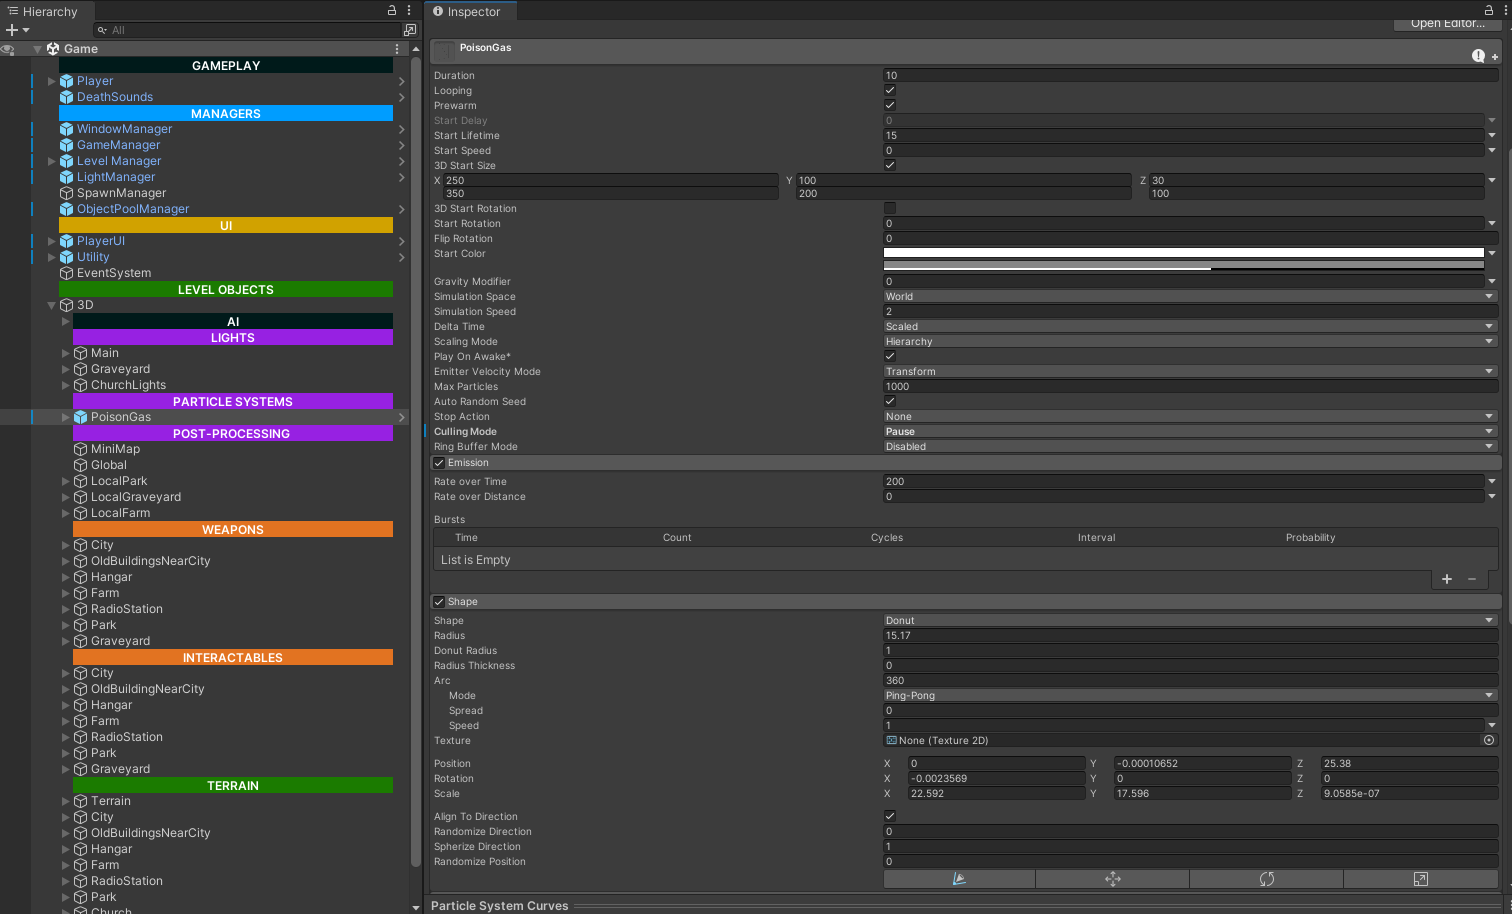
\includegraphics[width=1\linewidth]{Images/gaz1.PNG}
    \centering
    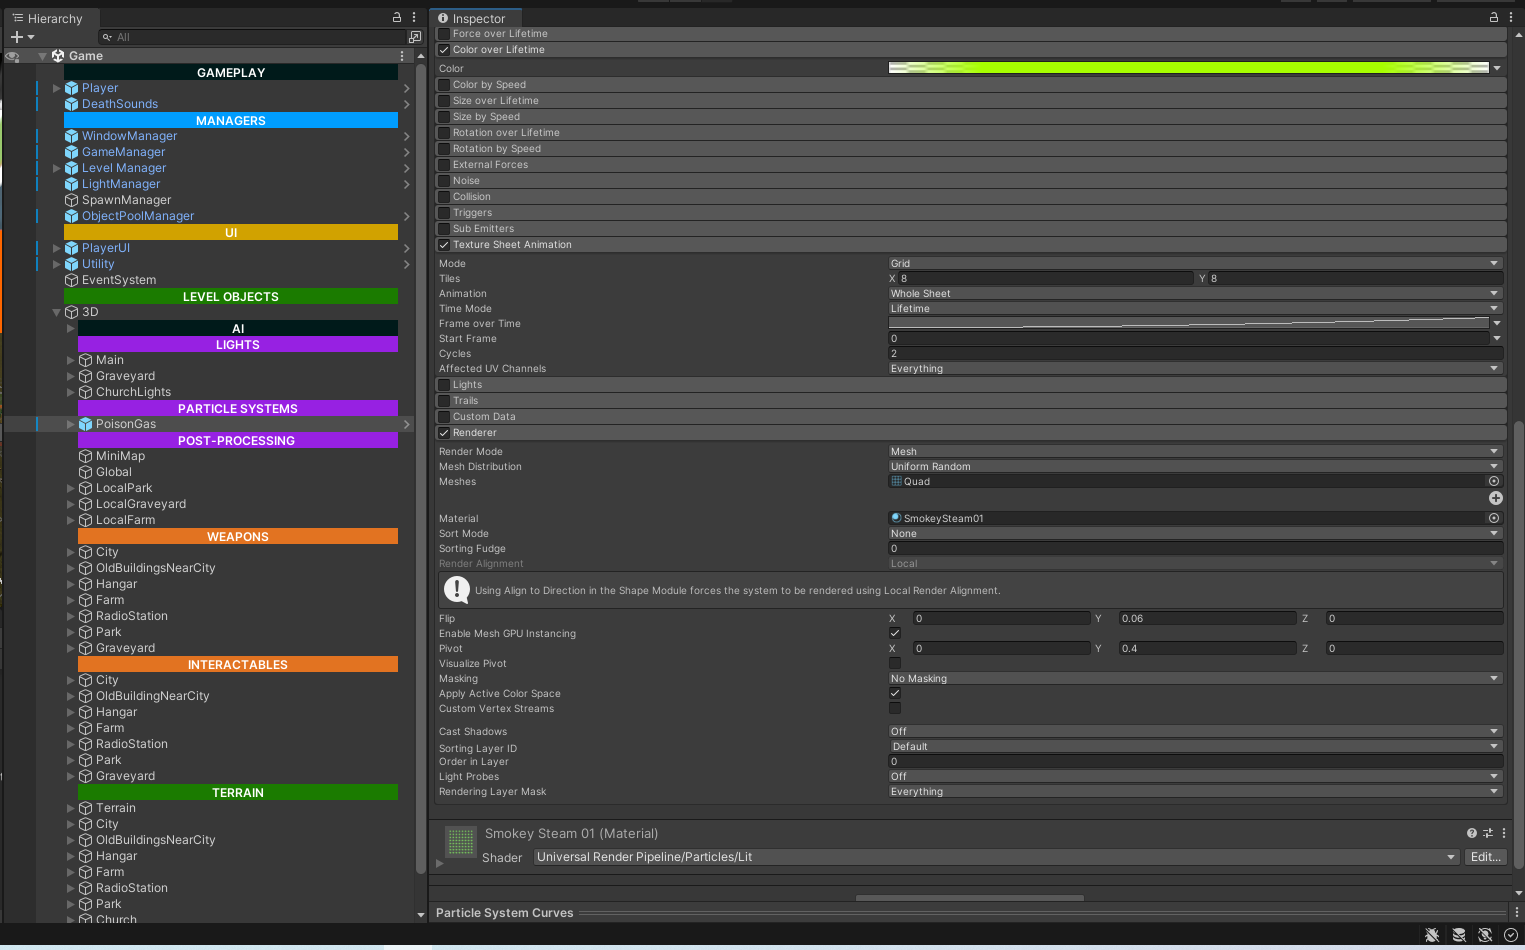
\includegraphics[width=1\linewidth]{Images/gaz2.PNG}
    \caption{Przedstawienie konfiguracji gazu}
\end{figure}
\FloatBarrier
\subsubsection{VFX}
\begin{itemize}
\item \texttt{Efekt podpalenia postaci:} Ten efekt pojawia się, gdy przeciwnik wejdzie w obszar pokryty ogniem z koktajlu Mołotowa. Postać staje się ognistą, co nie tylko wprowadza elementy wizualne, ale także może wpływać na mechanikę rozgrywki, dodając elementy takie jak obrażenia od ognia lub zmienione zachowanie postaci w płomieniach.
\begin{figure}[h]
    \centering
    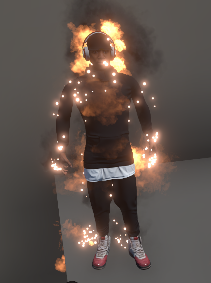
\includegraphics[scale=0.7]{Images/onFire.png}
    \caption{Efekt podpalenia w grze}
\end{figure}
\item \texttt{Efekt dymu:} Ten efekt aktywuje się w momencie użycia granatu dymnego. Tworzy gęsty dym, który może pełnić różne funkcje w grze, takie jak ukrywanie ruchów gracza przed przeciwnikami, zmiana taktyki lub tworzenie warunków do uniknięcia wykrycia. Jest to ważny element taktyczny wpływający zarówno na rozgrywkę, jak i na aspekty wizualne.
\begin{figure}[h]
    \centering
    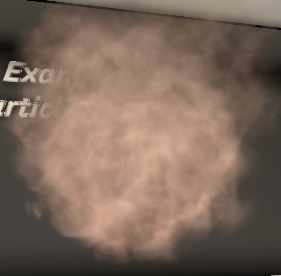
\includegraphics[scale=0.7]{Images/smoke.png}
    \caption{Efekt dymu w grze}
\end{figure}
\FloatBarrier
\end{itemize}